\chapter{Descrição dos Módulos}

A arquitetura da aplicação a desenvolver é definida por quatro módulos principais: Catálogo de clientes, Catálogo de produtos, Faturação Global e Vendas por Filial, cujas fontes de dados são três ficheiros de texto detalhados abaixo.
 
\paragraph{}
No ficheiro \textbf{Produtos.txt} cada linha representa o código de um produto vendável no hipermercado, sendo cada código formado por duas letras maiúsculas e 4 dígitos (que representam um inteiro entre 1000 e 1999), como no exemplo: 

\begin{verbatim}
AB9012
XY1185
BC9190
\end{verbatim}

O ficheiro de produtos contém cerca de 200.000 códigos de produto. 

\paragraph{}
No ficheiro \textbf{Clientes.txt} cada linha representa o código de um cliente identificado no hipermercado, sendo cada código de cliente formado por uma letra maiúscula e 4 dígitos que representam um inteiro entre 1000 e 5000, segue um exemplo: 

\begin{Verbatim}
F2916
W1219
F2915
\end{Verbatim}

O ficheiro de clientes contém cerca de 20.000 códigos de cliente. 

\paragraph{}
O ficheiro \textbf{Vendas\_1M.txt}, no qual cada linha representa o registo de uma venda efectuada numa qualquer das 3 filiais da Cadeia de Distribuição. Cada linha (a que chamaremos compra ou venda, o que apenas depende do ponto de vista) será formada por um código de produto, um preço unitário decimal (entre 0.0 e 999.99), o número inteiro de unidades compradas (entre 1 e 200), a letra \textbf{N} ou \textbf{P} conforme tenha sido uma compra \textbf{Normal} ou uma compra em \textbf{Promoção}, o código do cliente, o mês da compra (1 ... 12) e a filial (de 1 a 3) onde a venda foi realizada, como se pode verificar nos exemplos seguintes:
 
 \begin{Verbatim}
KR1583 77.72 128 P L4891 2 1
QQ1041 536.53 194 P X4054 12 3
OP1244 481.43 67 P Q3869 9 1
JP1982 343.2 168 N T1805 10 2
IZ1636 923.72 193 P T2220 4 2 
 \end{Verbatim}
 
O ficheiro de vendas inicial, \textbf{Vendas\_1M.txt} , conterá 1.000.000 (1 milhão) de registos de vendas realizadas nas 3 filiais da cadeia de distribuição. Existirão também os ficheiros  \textbf{Vendas\_3M.txt} e  \textbf{Vendas\_5M.txt} utilizados para as questões de performance da aplicação. 

\newpage 
\paragraph{}
A aplicação possuiu uma arquitectura tal como apresentado na figura seguinte, em que se identificam as fontes de dados, a sua leitura e os módulos de dados a construir: 

\begin{figure}[h!]
	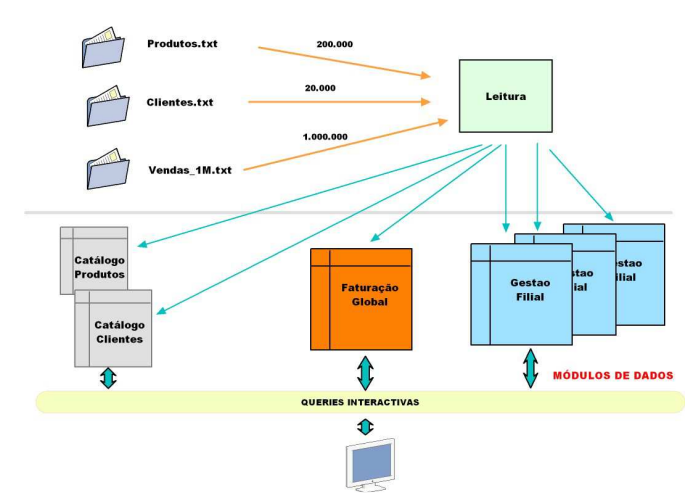
\includegraphics[scale=0.8]{arquiteturaproj.png}  
	\caption{Arquitetura da aplicação}  
\end{figure}


\section{Catálogo de Clientes}
É o módulo de dados onde são guardados os códigos de todos os clientes do ficheiro \textbf{Clientes.txt}, organizados por índice alfabético; 

\subsection{Clientes.h}

Módulo de dados onde são guardados os códigos de todos os clientes do ficheiro \textbf{Clientes.txt}. O array de árvores este que é um array de 26 posições cujos índices se encontram organizados alfabeticamente. Cada índice contém um apontador para uma árvore correspondente à letra respetiva desse índice.

Utilizamos uma estrutura 

\subsubsection{Tipos Opacos}


\begin{Verbatim}
typedef struct catalogo_clientes *CatClientes;
\end{Verbatim}

O typedef no ficheiro Clientes.h é a única informação que o utilizador têm relativamente à implementação de dados, não tendo acesso ao ficheiro .c dos clientes, não conseguindo conhecer a verdadeira implementação da estrutura AVL. Deste modo garantimos o encapsulamento de dados e a única forma de o utilizador interagir com o catálogo de clientes será através da API; 


\paragraph{}
\textbf{clientes.c}
\begin{verbatim}
struct catalogo_clientes{
ARVORE indices[27];
};
\end{verbatim}

Para guardar os clientes lidos a partir do ficheiro resolvemos usar  AVLs, pois  executa as operações de inserção, busca e remoção em tempo O(log n), sendo rápida  para aplicações que fazem uma quantidade excessiva de procuras, porém esta estrutura é um pouco mais lenta para inserção e remoção. Isso deve-se ao facto de as árvores AVL serem rigidamente balanceadas.


\subsubsection{/*API*/}
\begin{itemize}

\item CatClientes inicializa\_catalogo\_clientes() - Função que cria uma estrutura de clientes vazia;

\item void insertC(CatClientes c, char * valor) - insere um dado cliente na estrutura CatClientes, de maneira ordenada alfabeticamente; 

\item void cat\_remove\_cliente(CatClientes cat, char *str) - remove um cliente da estrutura CatCliente 

\item void free\_catalogo\_Clientes(CatClientes cat) - função que liberta todo o espaço ocupado pela estrutura CatClientes

\item int existeCliente (char *cliente,CatClientes cat) - função que verifica se um cliente existe
\item int numeroClientes(CatClientes cat) - função que conta todos os nodos

\item int numeroClientesLetra(CatClientes cat, char letra) - função que conta os nodos por que começam por determinada letra


\end{itemize}

\section{Catálogo de Produtos}

 Módulo de dados onde são guardados os códigos de todos os produtos do ficheiro \textbf{Produtos.txt}, organizados por índice alfabético, o que irá permitir, de forma eficaz, saber quais são os produtos cujos códigos começam por uma dada letra do alfabeto e saber quantos produtos são contabilizados. 


\subsection{Produtos.h}

\subsubsection{Tipos Opacos}
\begin{verbatim}
typedef struct catalogo_produtos *CatProdutos;
\end{verbatim}

Este typedef é a única informação que o utilizador tem relativamente à implementação de dados, não tendo acesso ao ficheiro .c dos produtos não consegue conhecer a verdadeira implementação da estrutura AVL. Assim, garantimos o encapsulamento de dados e a única forma de o utilizador interagir com o catálogo de produtos será através da API. 

\paragraph{}
\textbf{produtos.c}

\begin{verbatim}
struct catalogo_produtos{
ARVORE indices[27];
};
\end{verbatim}

 Para guardar os produtos lidos a partir do ficheiro utilizámos uma avl,

\subsubsection{/*API*/}

\begin{itemize}
	
\item CatProdutos inicializa\_catalogo\_produtos() - 
\item void insertP(CatProdutos c, char * valor);
\item void cat\_remove\_produto(CatProdutos cat, char *str);
\item void free\_catalogo\_produtos(CatProdutos cat);
\item int existeProduto (char *produto,CatProdutos cat);
\item int numeroProdutos(CatProdutos cat);
\item int numeroProdutosLetra(CatProdutos cat, char letra);
\item ARRAY listaProdutosLetra(CatProdutos cat, char l);
\end{itemize}


\section{Faturação Global}

Módulo de dados que contém as estruturas de dados responsáveis pela resposta a questões quantitativas que relacionam os produtos às suas vendas mensais, em modo Normal (N) ou em Promoção (P), para cada um dos casos guardando o número de vendas e o valor total de faturação de cada um destes tipos. Este módulo refecencia todos os produtos, mesmo os que nunca foram vendidos, não contém qualquer referência a clientes, mas é capaz de distinguir os valores obtidos em cada filial. 

\subsection{faturacao.h}

\subsubsection{Tipos Opacos}
\begin{Verbatim}
typedef struct faturacao *Faturacao;
typedef struct info *Info;
\end{Verbatim}

\textbf{faturacao.c}
\begin{verbatim}
struct faturacao{
int totalvendas[12];
float totalfaturado[12];
ARVORE produtos;
};

struct info{
char *code;
int vendasP[12][3];
int vendasN[12][3];
float faturadoN[12][3];
float faturadoP[12][3];
int quantidadeP[12][3];
int quantidadeN[12][3];
};
\end{verbatim}

Para guardar a informação relativa à faturação utilizámos um array de 12 AVLs, pois esta estrutura permite ordenar estruturas complexas de acordo com um método de comparação, separando pelos 12 meses. Como existe ordem alfabética, a AVL permite fazer procura rápida, preservando assim memória. 

\paragraph{}
AVL com informação do número de vendas e o seu valor distinguido por normal ou promoção, ordenada pelo código de produto

\subsubsection{/*API*/}

\begin{itemize}

\item	Faturacao inicializa\_faturacao() - A funcão inicializa\_faturacao aloca uma estrutura Faturacao e cria uma avl para os produtos, bem como inicializa os 12 nodos totalvendas e totalfaurado a zero; 

\item	void cont\_regista\_produto(Faturacao fat, char *prod) - A funcão cont\_regista\_produto, dada a estrutura faturacão e um id de produto, insere-o através da funcão avl\_insert; 

\item	void cont\_insere\_venda(Faturacao fat, char *produto, int q, float preco, char M,int mes, int filial) - A funcão cont\_insere\_venda, dada a estrutura faturacão, atualiza as vendas, quantidades e faturado conforme o produto em questão ser Promocão (P) ou Normal (N); 

\item	void cont\_remove\_produto(Faturacao fat, char *produto) - A funcão cont\_remove\_produto remove um produto da Faturacao passados ambos por parametro. Inicialmente calcula o id do produto através da funcão fat\_procura\_info para depois eliminar o produto em questão através da funcão avl\_delete e logo a seguir faz free ao nodo eliminado através da funcão free\_info;

\item	void free\_faturacao(Faturacao fat) - A funcão free\_faturacao elimina todos os nodos da faturacao através da funcão avl\_destroy e faz free à estrutura faturacao passada por parâmetro;

\item	float getTotalFatPFilialX (char* prod,int mes,Faturacao fat, int filial) - A funcão getTotalFatPFilialX vai calcular o total faturado no modo Promocão (P) de um dado produto, num determinado mês e em determinada filial; 

\item	float getTotalFatNFilialX (char* prod,int mes,Faturacao fat, int filial) - A funcão getTotalFatNFilialX vai calcular o total faturado no modo Normal (N) de um dado produto, num determinado mes e em determinada filial;

\item	int getVendasNFilialX (char* prod,int mes,Faturacao fat, int filial) - A funcão getVendasNFilialX calcula o nr de vendas em modo Normal (N) de um produto num determinado mês e filial. Inicialmente vai buscar o produto através do seu id, se o encontrar devolve o nr de vendas nas condicões anteriores; 

\item	int getVendasPFilialX (char* prod,int mes,Faturacao fat, int filial) - A funcão getVendasPFilialX calcula o nr de vendas em modo Promocao (P) de um produto num determinado mês e filial. Inicialmente vai buscar o produto através do seu id, se o encontrar devolve o nr de vendas nas condicões anteriores; 

\item	int getQuantidadeNFilialX (char* prod,int mes,Faturacao fat, int filial) - A funcão getQuantidadeNFilialX calcula a quantidade vendida em modo Normal (N) de um determinado produto num dado mês e filial;

\item	int getQuantidadePFilialX (char* prod,int mes,Faturacao fat, int filial) - A funcão getQuantidadePFilialX calcula a quantidade vendida em modo Promocão (P) de um determinado produto num dado mês e filial. Inicialmente vai buscar o nodo do produto através do id do produto e retorna finalmente a quantidade vendida; 

\item	ARRAY naoCompradosFilial(Faturacao fat, int filial) - A funcão naoCompradosFilial percorre a estrutura da faturacao numa dada filial em todos os meses através do Traverser t, e verificia se este foi ou não comprado,se foi nada faz, se não insere-o num array a. No final faz free ao Traversser t e retorna o novo array; 
\item	ARRAY naoComprados(Faturacao fat) - A funcão naoComprados percorre  a estrutura da faturacao em todas as filiais e em todos os meses através do Traverser t, e verificia se este foi ou não comprado,se foi nada faz, se não insere-o num array a. No final faz free ao Traversser t e retorna o novo array; 
\item	int totalVendasMeses(Faturacao fat, int a, int b) - A funcão totalVendasMeses calcula o total de vendas num determinado intervalo de meses;

\item	float totalFatMeses(Faturacao fat, int a, int b) - A funcão totalFatMeses calcula o total faturado num dado intervalo de meses; 

\item	ARRAY nMaisVendidos(Faturacao fat, int n) - A funcão nMaisVendidos calcula os n produtos mais vendidos de todas as filiais através de um traversser t. Inicialza dois arrays a e b através da funcão inicializa\_array . Copia os elementos do tipo Info para o array a, ordena-o através da funcão ordena e depois devolve o array b com os elementos ids dos produtos do array já ordenados; 

\item	int getQuantidadeFilial(Faturacao fat, char*prod, int filial) - A funcão getQuantidadeFilial calcula a quantidade vendida de um determinado produto através do seu id de produto numa determinada filial em todos os meses. 
	
\end{itemize}


\section{Gestão da Filial}

Módulo de dados que, a partir dos ficheiros lidos, contém as estruturas de dados adequadas à representação dos relacionamentos, fundamentais para a aplicação, entre produtos e clientes, ou seja, para cada produto, saber quais os clientes que o compraram, quantas unidades cada um comprou, em que mês e em que filial.

 Para a estruturação optimizada dos dados deste módulo de dados tivemos em atenção que pretendemos ter o histórico de vendas organizado por filiais para uma melhor análise, nunca esquecendo que existem 3 filiais nesta cadeia. 

\subsection{Filial.h}

\subsubsection{Tipos Opacos}
\begin{Verbatim}
typedef struct filial *Filial;
typedef struct icliente *Icliente;
typedef struct iprodutos *Iprodutos;
\end{Verbatim}

\textbf{Filial.c}
\begin{verbatim}
struct filial{
ARVORE infoCliente;
};

struct icliente{
char *cliente;
int quantidade[12];
ARVORE infoprodutos[2];
};

struct iprodutos{
char *prod;
int quantidadeT;
float gastouT;
int quantidade[12];
float gastou[12];
};
\end{verbatim}

Estrutura de cliente que contém .... 

Estrutura de produtos que contém ...........


\subsubsection{/*API*/}

\begin{itemize}
\item	Filial inicializa\_filial() - Inicializa a estrutura da filial; 

\item	void fil\_regista\_cliente(Filial fil, char *cliente) - Insere um cliente na filial; 

\item 	\textbf{void fil\_insere\_prod(Filial fil, char *cliente, char *produto,int q, int mes, float preco, char p)} - A funcão fil\_insere\_prod insere  um produto comprado por um dado cliente num dado mês, se o produto já tiver sido inserido a quantidade =quantidadeAntiga+quantidadeComprada, aumenta também o dinheiro gasto nesse produto. Senão tiver sido inserido a quantidade=quantidadeComprada e o 
preco=precoComprado; 
 
\item	\textbf{int getQuantidadeMesCliente(Filial fil, char *cliente, int mes)} - A funcão getQuantidadeMesCliente retorna a quantidade dos produtos comprados por um dado cliente, num dado mês. Para tal, procura um cliente numa dada filial através da funcão fil\_procura\_cliente, retornando a quantidade comprada  desse mês; 

\item	ARRAY naoCompraram(Filial fil);
\item	ARRAY compraram(Filial fil);
\item	\textbf{void clientesCompraram(Filial fil,ARRAY a)} - A funcão clientesCompraram remove do array todos os clientes que não compraram nenhum produto numa filial passada por parâmetro. Para isso cria um Traversser t percorredo a estrutura dos clientes, somando a quantidade comprada em cada mês, se esta for zero então remove o cliente do array através da funcão remove\_posicão; 
\item	\textbf{void free\_filial(Filial fil)} - A função free\_filial elimina todos os nodos da filial através da funcão avl\_destroy e faz  free à estrutura filial passada por parâmetro; 
\item	\textbf{ARRAY topMaisGastou(ARRAY a)} - A funcão topMaisGastou irá calcular os 3 produtos que um cliente mais gastou retornando-os num array. Para isso recebe um array de Produtos comprados por um dado cliente, ordena esse array a (passado por parâmetro) e insere as chaves num array b, retornando-o; 
\item	ARRAY clientesCompraramProduto(Filial fil, char* produto) - Retorna a lista de clientes que compraram um determinado produto; 

\item	int comprouProdutoN(Filial fil, char* cliente, char* produto) - A funcão comprouProdutoN verifica se um dado cliente comprou um dado produto em regime normal; 

\item	int comprouProdutoP(Filial fil, char* cliente, char* produto) - função que diz se um dado cliente comprou um dado produto em promoção; 

\item	int getNumClientesFilial(Filial fil, char* produto) - diz quantos clientes compraram um determinado produto; 

\item	void getIProdMes(Filial fil, char* cliente, int mes, ARRAY a) - Para um dado cliente e para um mês, inser a informacao, dos produtos que o cliente comprou nesse mês numa dada filial; 
\item	ARRAY extraiPorQuantidade(ARRAY a,int mes) - Devolve uma lista de produtos mais comprados, por quantidade, de um dado mês; 
\item	void removeNaoCompraram(Filial fil, ARRAY a);
\item	void removeCompraram(Filial fil, ARRAY a);
\end{itemize}


\chapter{Main}

O programa é controlado pelo ficheiro leitura.c. Este que invoca as funções que estão inseridas no ficheiro querie.c este que carrega os ficheros de produtos, clientes e vendas em variáveis do tipo FILE,  também é responsável pela interação com o utilizador.


 
Depois, são usadas funções derivadas dos vários módulos para carregar os ficheiros em memória nas devidas estruturas. Após a colocação em memória, é chamada a função auxiliar querie, que servirá para selecionar a querie que o utilizador pretende executar. Escolhida a querie, com o auxílio de um switch, temos acesso a funções que invocam a função que faz exatamente o que a querie pede e mostra ao utilizador os resultados pretendidos.


\chapter{Interface do utilizador}
Quando o utilizador executa o programa é-lhe pedido que escolha qual o documento de texto que pretende analisar, como podemos observar na figura seguinte: 

\begin{figure}[h!]
	\centering
	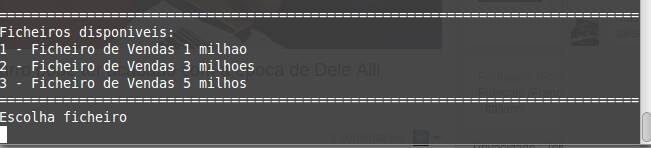
\includegraphics[scale=0.4]{1querie.png}  
	\caption{Escolha do ficheiro de vendas a analisar}  
\end{figure}

O ficheiro é carregado e de seguida aparece um menu com 12 opções, referentes às 12 queries do projeto, sendo que decidimos usar o [0] para sair do GereVendas. O objetivo é que o utilizador prima a tecla correspondente à opção do menu pretendida.

\begin{figure}[h!]
	\centering
	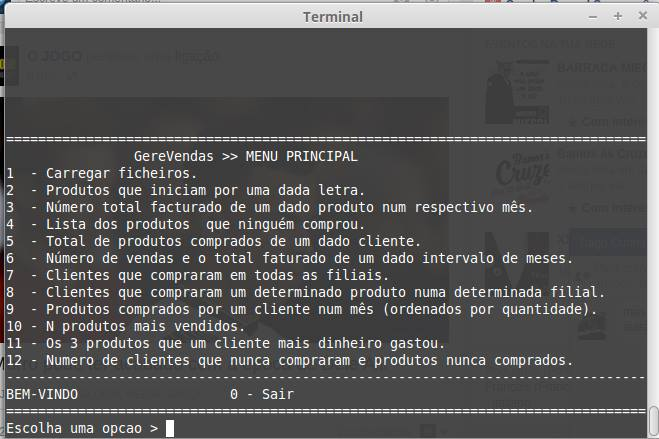
\includegraphics[scale=0.6]{menu.png}  
	\caption{Menu principal da aplicação}  
\end{figure}


\chapter{Resultados e comentários sobre os testes de performance}
Depois de desenvolver e codificar todo o projeto foi-nos proposto realizar alguns testes de performance que consistem em comparar os tempos de execução das queries 8, 9, 10, 11 e 12 usando os ficheiros Vendas\_1M.txt ( 1000 000 vendas), Vendas\_3M.txt (3 milhões de vendas) e Vendas\_5M.txt (5 milhões de vendas).
Uma vez que a quantidade de vendas vai aumentando de ficheiro para ficheiro é aceitável que os tempos de execução para os carregar aumente.


\begin{figure}[h!]
	\centering
	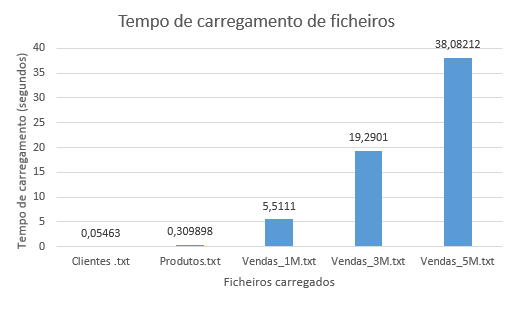
\includegraphics[scale=0.8]{grafcarregamento.png}  
	\caption{Gráfico do tempo de carregamento dos ficheiros de clientes, produtos e os 3 ficheiros de vendas}  
\end{figure}

Comparando os valores de execução das queries pretendidas, como podemos observar nos respetivos gráficos apresentados,

  	\begin{minipage}{0.45\linewidth}
  		\begin{figure}[H]
  			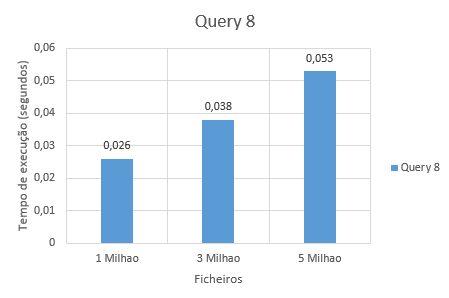
\includegraphics[width=\linewidth]{grafq8}
  			\caption{Tempos de execução da querie 8 para a filial 1 e o produto GI1298}
  		\end{figure}
  	\end{minipage}
  	\hspace{0.05\linewidth}
  	\begin{minipage}{0.45\linewidth}
  		\begin{figure}[H]
  			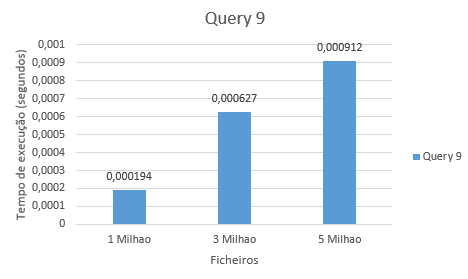
\includegraphics[width=\linewidth]{grafq9}
  			\caption{Tempos de execução da querie 9 para o cliente Z5000 para o mês 1}
  		\end{figure}
  	\end{minipage}
  	
  	\begin{minipage}{0.45\linewidth}
  		\begin{figure}[H]
  			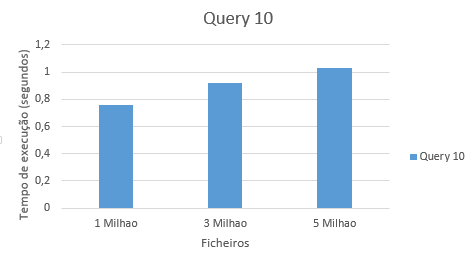
\includegraphics[width=\linewidth]{grafq10}
  			\caption{Tempos de execução da querie 10, para os 10 produtos mais vendidos}
  		\end{figure}
  	\end{minipage}
  	\hspace{0.05\linewidth}
  	\begin{minipage}{0.45\linewidth}
  		\begin{figure}[H]
  			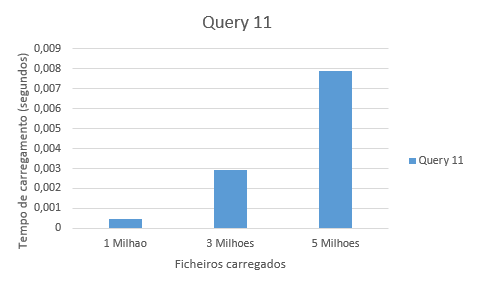
\includegraphics[width=\linewidth]{grafq11}
  			\caption{Tempos de execução da querie 11 para o cliente Z5000}
  		\end{figure}
  	\end{minipage}
  	
  	
  	\begin{figure}[h!]
  		\centering
  		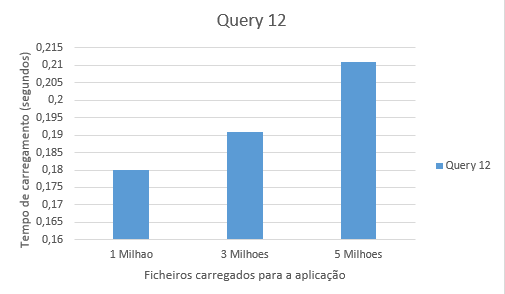
\includegraphics[scale=0.7]{grafq12}  
  		\caption{Gráfico do tempo de carregamento da querie 12 - nr de clientes que nunca compraram e produtos nunca comprados}  
  	\end{figure}





\chapter{Makefile e Grafo de dependências}
A makefile permite correr todo o software escrevendo apenas \textit{“make”} no terminal. Posto isto, apresenta-se a makefile utilizada cujas flags utilizadas como opção de compilação são –Wall –Wextra –ansi – pedantic –O2.
Possui ainda a opção “make clean” que elimina todos os “.o” que foram criados quando se compilou o software.

\begin{figure}[h!]
	\centering
	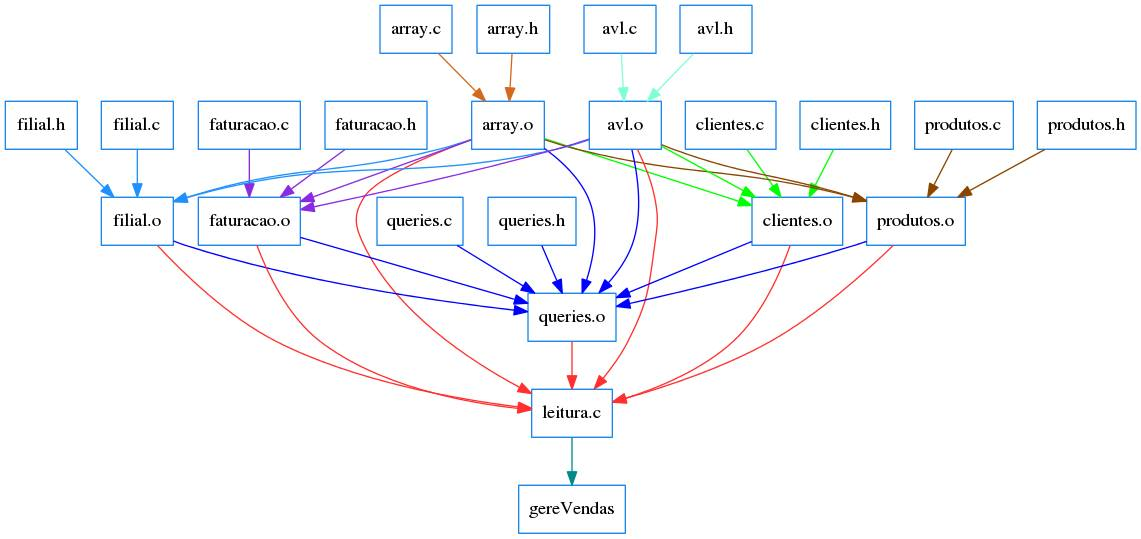
\includegraphics[scale=0.4]{grafodependencias.png}  
	\caption{Grafo de depêndencias}  
\end{figure}

\begin{verbatim}
objects = array.o avl.o clientes.o faturacao.o filial.o \
produtos.o queries.o 

CFLAGS=-Wall -ansi -pedantic -O2

all:
make clean
make produtos
make array
make avl
make clientes
make faturacao
make filial
make queries
make leitura

leitura: src/leitura.c array.o avl.o clientes.o faturacao.o filial.o
 produtos.o queries.o 
gcc src/leitura.c array.o avl.o clientes.o faturacao.o filial.o
 produtos.o queries.o $(CFLAGS) -o gereVendas -lm

queries: src/queries.c src/headers/queries.h
gcc src/queries.c -c $(CFLAGS)

clientes: src/clientes.c src/headers/clientes.h
gcc src/clientes.c -c $(CFLAGS)

produtos: src/produtos.c src/headers/produtos.h
gcc src/produtos.c -c $(CFLAGS)

array: src/array.c src/headers/array.h
gcc src/array.c -c $(CFLAGS)

faturacao: src/faturacao.c src/headers/faturacao.h
gcc src/faturacao.c -c $(CFLAGS)

filial: src/filial.c src/headers/filial.h
gcc src/filial.c -c $(CFLAGS)

avl: src/avl.c src/headers/avl.h
gcc src/avl.c -c $(CFLAGS)

.PHONY : clean
clean :
rm -f gereVendas
rm -f $(objects)
rm -f gesval
\end{verbatim}
